\documentclass[11pt,a4paper]{article}
\usepackage[utf8]{inputenc}
\usepackage[ngerman]{babel}
\usepackage{csquotes}
\usepackage{graphicx}
\usepackage{geometry}
\usepackage{hyperref}
\usepackage{subfiles}
\usepackage{amssymb}
\usepackage{amsmath}
\usepackage{tabularx}
\usepackage{listings}
\usepackage[acronyms, toc]{glossaries}
\usepackage{colortbl}
\usepackage{color}
\usepackage[rgb]{xcolor}
\usepackage{afterpage}
\usepackage{pdflscape} 
\usepackage[style=apa, backend=biber]{biblatex}

\usepackage{tikz}
% \usepackage{indentfirst} 
% \usepackage[
%     colorlinks=true, 
%     linkcolor=blue,
%     urlcolor=blue,
%     citecolor=blue,
%     anchorcolor=blue
% ]{hyperref}

\usetikzlibrary{matrix, positioning, calc, fit}

\makeglossaries

\newglossaryentry{wake-up-word}{
	name={Wake-up Wort},
  	description={Ein Wake-up Wort ist ein Wort oder eine Wortsequenz, die ein System aktiviert.},
  	plural={Wake-up Wörter}
}

\newacronym{ai}{AI}{Künstliche Intelligenz}



\addbibresource{references.bib}
\geometry{a4paper, total={170mm,257mm}, left=20mm, top=20mm}
\definecolor{ba-gray}{rgb}{0.9,0.9,0.9}

\newcommand\blankpage{%
	\null
	\thispagestyle{empty}%
	\addtocounter{page}{-1}%
	\newpage}

\newcommand\redpage{%
	\newpage
	\pagecolor{red}
	\blankpage
	\afterpage{\nopagecolor}}


\definecolor{codeblack}{rgb}{0.1,0.1,0.23}
\definecolor{codegreen}{rgb}{0.2,0.5,0.1}
\definecolor{codepurple}{rgb}{0.5,0.0,0.5}
\definecolor{backcolour}{rgb}{0.95,0.95,0.95}
\definecolor{codered}{rgb}{0.7,0.1,0.2}

\lstset{
	language=Python,
	basicstyle=\ttfamily\footnotesize, % footnotesize gibt eine kleinere Schriftgrösse
	backgroundcolor=\color{white},
	commentstyle=\color{codegreen},
	keywordstyle=\color{codered},
	numberstyle=\tiny\color{codegray},
	stringstyle=\color{codepurple},
	identifierstyle=\color{codeblack},
	showstringspaces=false,
	numbers=none,
	captionpos=b,
	frame=none,
	rulecolor=\color{black},
	aboveskip=1em, % Abstand über dem Code
	belowskip=1em  % Abstand unter dem Code
}


\title{
{\LARGE Bachelorarbeit}\\[2em]
{\textbf{Integration einer Sprachsteuerungsfunktion {\break} in Mobile Apps}}
}
\author{Rubén Nuñez}
\date{Herbstsemester 2023}

\begin{document}

\maketitle
\thispagestyle{empty} %Keine Seitennummerierung auf der start Seite
\newpage

\section*{Bachelorarbeit an der Hochschule Luzern -- Informatik}
\subfile{affidavit.tex}
\newpage

\newpage \section*{Abstract}
Das Problem dieser Arbeit ist im wesentlichen die Erkennung von Wake-up Wörter innerhalb
des Kontext einer App. Grundsätzlich ist es unüblich, dass mobile Apps eine
integrierte Sprachsteuerungsfunktion anbieten. 


\newpage
\tableofcontents

\newpage

\newpage \section{Problem, Fragestellung, Vision}
\subsection{Problemstellung}
Sprachsteuerungstechnologien haben ein grosses Potenzial und werden bisher vor allem als 
Sprachsteuerungsassistenten genutzt. Während es etablierte Sprachassistenten wie Siri, Google 
oder Alexa gibt, fehlt es an Lösungen für eine integrierte Sprachsteuerung in Mobile Apps, 
insbesondere in Bezug auf das Erkennen von \gls{wake-up-word}. Daher gibt es eine Lücke
zwischen eigenen Sprachassistenten und Mobile Apps. Diese Lücke soll mit dieser Arbeit 
geschlossen werden.

\subsection{Fragestellung}
Wie kann eine integrierte Sprachsteuerung für eine Mobile App entwickelt werden, die speziell 
das Erkennen von \glspl{wake-up-word} oder \textit{Wake-up Wortsequenzen} ermöglicht?


\subsection{Vision}
Als Vision dieser Arbeit soll eine Grundlage geschaffen werden, um ein \textit{Wake-up} Wort 
oder eine Sequenz von \textit{Wake-up Wörtern} in der akustischen Sprache erkennen zu können.
Dabei sollen Methoden und Werkzeuge aus dem Bereich des Machine Learnings verwendet werden.
Zum anderen soll diese Erkenntnise in eine mobile Plattform wie iOS oder Android integriert 
werden. Für den Rahmen dieser Arbeit genügt die Integration in eine der genannten Plattformen. 
Weiterhin ist es ein Anliegen dieser Arbeit, dass das Thema Datenschutz und die ethischen Aspekte 
zu berücksichtigen sind.


\newpage \section{Grundlagen}
Um diese Arbeit fundiert anzugehen, ist ein Verständnis der Grundlagen in den Bereichen
Audioverarbeitung und Machine Learning essenziell. Daher wird in diesem Kapitel ein Überblick
über die wichtigsten Themen gegeben.

\subsection{Audio}
In der digitalen Welt repräsentiert Audio Schallwellen, die durch eine Reihe von numerischen Werten
dargestellt werden. (\cite[p.9]{somberg2019audioapi}) beschreibt Audio als: \glqq Fundamentally,
audio can be modeled as waves in an elastic medium. In our normal everyday experience, the elastic
medium is air, and the waves are air pressure waves.\grqq \ Audiosignale werden durch die Funktion
\(A(t)\) repräsentiert, wobei \(t\) die Zeit und \(A(t)\) die Amplitude zum
Zeitpunkt \(t\) angibt. Die Amplitude ist die Stärke des Signals und die Zeit repräsentiert die
Position des Signals in der Zeit. Diese Betrachtung ist vor allem in der Elektrotechnik
von Bedeutung, da die Amplitude als Spannung angesehen werden kann. Grundsätzlich ist Audio ein
kontinuierliches Signal. In der digitalen Welt können wir jedoch nur diskrete Werte darstellen.
Daher wird das kontinuierliche Signal in diskrete Werte umgewandelt. Dieser Vorgang wird als
\textit{Sampling} bezeichnet (\cite[Chapter~3.1]{tarr2018hackaudio}).


\subsubsection{Sampling}
Ein früher Ansatz zur digitalen Darstellung von analogen Signalen war die Pulse-Code-Modulation
(PCM). Dieses Verfahren wurde bereits in den 1930er Jahren von Alec H. Reeves entwickelt,
parallel zum Aufkommen der digitalen Telekommunikation (\cite[p.~57]{deloraine1965pcm}).
Im Grundsatz wird es heute noch in modernen Computersystemen nach dem gleichen Verfahren angewendet.

\noindent \newline
Es folgt eine formelle Definition von Sampling. Ein kontinuierliches Signal \(A(t)\)
wird in bestimmten Zeitintervallen \(T_s\) gesampelt. Diese Zeitintervalle werden auch als
Sampling-Periode bezeichnet. Die Sampling-Rate \(F_s = \displaystyle\frac{1}{T_s}\) gibt die Anzahl
der Samples pro Sekunde an. Angenommen wir haben ein Signal mit einer Sampling-Periode
von \(T_s = 0.001\). Um nun die Sampling-Rate zu berechnen, müssen wir den Kehrwert der
Sampling-Periode berechnen. \(F_s = \displaystyle\frac{1}{0.001} = 1000\). Somit erhalten wir eine
Sampling-Rate von \(1000\) Samples pro Sekunde. Nun typische Sampling-Raten sind \(44100\) Hz
oder \(48000\) Hz. Bei Sampling-Raten wird die Einheit \textit{Hertz} verwendet. Ein Hertz entspricht
einer Frequenz von einem Sample pro Sekunde. Ein weiter wichtiger Begriff ist die
\textit{Nyquist-Frequenz}. Die Nyquist-Frequenz \(F_n\) ist die Hälfte der Sampling-Rate.
Also \(F_n = \displaystyle\frac{F_s}{2}\). Die Idee hinter der Nyquist-Frequenz ist, dass die
Sampling-Rate mindestens doppelt so hoch sein muss wie die höchste Frequenz des Signals. Wenn diese
Eigenschaft erfüllt ist, kann das Signal ohne Informationsverlust rekonstruiert werden
(\cite[Chapter~3.1]{tarr2018hackaudio}). Mehr dazu folgt im Unterkapitel
\textit{Fourier-Analyse}.

\noindent \newline
Weiter ist es wichtig zu verstehen, dass ein Sample ein diskreter Wert ist. Und dieser wird in
digitalen Systemen durch eine bestimmte Anzahl von Bits dargestellt. Die Anzahl der Bits wird
als \textit{Bit-Depth} bezeichnet. Die Bit-Depth bestimmt die Auflösung des Signals. Typische
Bit-Depth Werte sind \(16\) oder \(24\) Bit (\cite[p.10]{somberg2019audioapi}).

\subsubsection{Frames, Channels, Buffers}
Ebendfalls wichtig ist das Verständnis von Frames, Channels und Buffers. Da diese Arbeit sich mit
Audio-Systemen beschäftigt, ist es wichtig, die Begriffe \textit{Frame}, \textit{Channel} und
\textit{Buffer} zu verstehen. Fangen wir mit dem Begriff \textit{Channel} an. Ein Channel kann als
ein einzelnes Audio-Signal angesehen werden. Ein Mono-Signal hat genau nur einen Channel. Ein
Stereo-Signal hat zwei Channels. Ein Surround-Signal hat mehr als zwei Channels. usw.
Nun zum Begriff \textit{Frame}. Ein Frame entspricht einem Sample pro Channel. Weiter sind Frames
in Buffers organisiert. Ein Buffer ist eine Sammlung von Frames. Typischerweise werden Buffers in
Grössen von \(64\), \(128\), \(256\), \(512\) oder \(1024\) Frames organisiert. Die Abbildung
\ref{fig:frames_channels_buffers} zeigt die Beziehung zwischen Frames, Channels und Buffers.
Die Abbildung wurde basierend auf (\cite[p.10]{somberg2019audioapi}) erstellt und verdeutlicht die
Beziehung zwischen Frames, Channels und Buffers.

\begin{figure}[h]
	\centering
	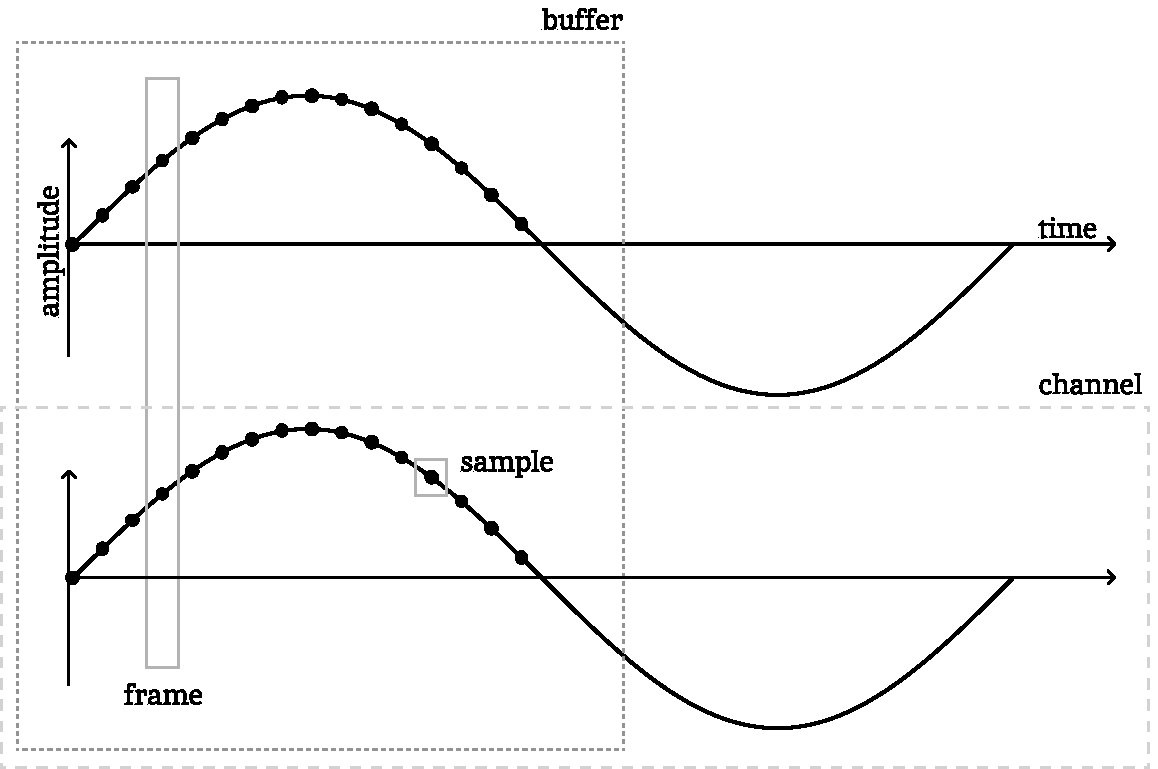
\includegraphics[width=0.7\linewidth]{img/audio-nutshell.pdf}
	\caption{Frames, Channels und Buffers}
	\label{fig:frames_channels_buffers}
\end{figure}

\subsubsection{Buffers im Detail}
Ein Buffer im Kontext von Audio ist eine aufeinanderfolgende Sammlung von Frames. Die bereits
angesprochene Grösse eines Buffers bestimmt im wesentlichen die Latenzzeit des Systems. Kleine
Buffer-Grössen haben eine geringe Latenzzeit, während grosse Buffer-Grössen eine hohe Latenzzeit
haben (\cite[p.10]{somberg2019audioapi}). Der Trade-Off ist dass kleine Buffer-Grössen
zu einer höheren CPU-Auslastung führen, während bei grossen Buffer-Grössen das nicht der Fall ist.
Das liegt daran, dass bei kleinen Buffer-Grössen die CPU häufiger aufgerufen wird, um die Buffers
zu verarbeiten.

\noindent \newline
Nun betrachten wir die mögliche Anordnung eines Buffers, wie in den folgenden Abbildungen
dargestellt. Es gibt zwei Möglichkeiten, wie Buffers angeordnet werden
können: \textit{Interleaved} und \textit{Non-Interleaved}. Bei der \textit{Interleaved}-Anordnung
werden die Samples der einzelnen Channels nacheinander in sequentieller Reihenfolge in den Buffer
geschrieben. Im Gegensatz dazu werden bei der \textit{Non-Interleaved}-Variante die Samples
eines Channels nacheinander in den Buffer geschrieben, bevor die Samples des nächsten Channels
hinzugefügt werden. Dieser Vorgang wird für jeden Channel wiederholt. Die Tabelle
\ref{tab:frames_buffers} zeigt die Unterschiede zwischen den beiden Anordnungen. Jede Zelle der
Tabelle entspricht einem Sample. L und R stehen exemplarisch für die Channels Left und Right.
Die erste Zeile entspricht der \textit{Interleaved}-Anordnung und die zweite Zeile der
\textit{Non-Interleaved}-Anordnung. Die Abbildung wurde basierend auf
(\cite[p.11]{somberg2019audioapi}) erstellt.

\begin{table}[h]
	\centering
	\begin{tabularx}{\textwidth}{|X|X|X|X|X|X|X|X|}
		\hline
		L & R & L & R & L & R & L & R \\
		\hline
		L & L & L & L & R & R & R & R \\
		\hline
	\end{tabularx}
	\caption{Frames in Interleaved und Non-interleaved Buffers}
	\label{tab:frames_buffers}
\end{table}

\noindent
Mit diesem Wissen kennen wir nun die Unterschiede zwischen den beiden Anordnungen. Für die
Anwendung ist es wichtig zu verstehen, mit welcher Anordnung die verwendete API arbeitet.

\subsection{Audio APIs}
Audio APIs sind im Bereich der Audioverarbeitung von essentieller Bedeutung. Sie bieten eine
Schnittstelle, welche den Zugriff auf vielfältige Audiofunktionen erlaubt. Ohne solche APIs müssten 
Entwickler die Audioverarbeitung von Grund auf neu implementieren. 

\noindent \newline
In der Erarbeitungsphase dieser Arbeit kristallisierten sich zwei primäre Anwendungsgebiete heraus. 
Erstens die intensive Auseinandersetzung mit Audioverarbeitung in Python, um tieferes Verständnis 
für die Materie zu entwickeln. Zweitens die Notwendigkeit, eine Audio API in eine mobile 
Applikation zu integrieren. Im Kontext dieser Arbeit werden sie als \textit{Audio API für Analyse} 
und \textit{Audio API für Integration} bezeichnet.

El sol es grande 

\noindent \newline
Im Bereich der \textit{Analyse} fiel die Wahl auf folgende APIs:

\begin{itemize}
\item \textbf{PyAudio:} Eine verbreitete Schnittstelle in Python zur Audioverarbeitung.
\item \textbf{SoundDevice:} Eine vielseitige Python-Bibliothek für Audioverarbeitungsaufgaben.
\item \textbf{librosa:} Eine Bibliothek, die speziell auf die Analyse von Audiosignalen 
ausgerichtet ist.
\end{itemize}

\noindent
Im Kontext der \textit{Integration} standen folgende APIs im Fokus:

\begin{itemize}
	\item \textbf{AVAudioEngine:} Eine leistungsfähige Schnittstelle primär für die Plattformen iOS 
    und macOS.
	\item \textbf{AudioTrack:} Eine spezialisierte API für Audioanwendungen auf Android-Geräten.
\end{itemize}

\noindent
Die folgenden Abschnitte werden tiefer auf die jeweiligen Eigenschaften und Möglichkeiten dieser 
APIs eingehen, insbesondere im Hinblick darauf, wie sie sich für die Aufnahme, Wiedergabe und 
Echtzeitverarbeitung von Audiodaten eignen.

\subsubsection{Audio API für Analyse}
Python zeichnet sich durch eine beeindruckende Auswahl an Bibliotheken für datenanalytische Aufgaben 
aus, zu denen auch NumPy, SciPy, Pandas und Matplotlib gehören. In dieser Arbeit wurde zunächst 
\textbf{PyAudio} in Erwägung gezogen. PyAudio ist als Schnittstelle zur PortAudio-Bibliothek 
bekannt, die plattformübergreifende Audioverarbeitungsfunktionen bereitstellt. Trotz ihrer 
intuitiven Funktionen für Aufnahme und Wiedergabe wurde PyAudio letztlich aufgrund von 
Inkompatibilitäten mit der gewählten Entwicklungsumgebung verworfen.
TODO: PyAudio/SoundDevice/librosa vergleichen

\subsubsection{Audio API für Integration}
TODO: AVAudioEngine, AudioTrack und kurze Codebeispiele

\newpage \subsection{Fourier-Analyse}
Die Fourier-Analyse befasst sich mit der Zerlegung von Funktionen in Frequenzkomponenten. Die
Fourier-Analyse ist ein wichtiges Konzept in der Signalverarbeitung und findet breite Anwendung
in der Audioverarbeitung. Daher ist ein Grundverständnis für diese Arbeit relevant.

\subsubsection{Fourier-Transformation}
Die Fourier-Transformation ist ein zentrales Werkzeug der Fourier-Analyse. Sie ermöglicht die
Zerlegung von Funktionen in ihre Frequenzkomponenten und die Rekonstruktion von Funktionen aus
diesen Komponenten. Dies wird als Fourier-Analyse und Fourier-Synthese bezeichnet. Dieses Konzept
wird auch von Prof. Dr. Weitz in seinem Video zu Fourier-Analyse erläutert
(\cite[2:20]{weitz2023fourier}). Mathematisch ausgedrückt wird die kontinuierliche
Fourier-Transformation eines Signals \( f(t) \) wie folgt definiert
(\cite[Chapter~5]{hansen2014fourier}):

\begin{equation*}
	F(\omega) = \int_{-\infty}^{\infty} f(t) e^{-i \omega t} \, dt
	\label{eq:fourier_transform}
\end{equation*}

\noindent
\(F(\omega)\) ist die Fourier-Transformation von \(f(t)\)
(\cite[49:27]{weitz2023fourier}). Als kleines Rechenbeispiel betrachten wir die
Fourier-Transformation der Rechteckfunktion \( \text{rect}(x) \), die wie folgt definiert ist:

\[
	\text{rect}(x) =
	\begin{cases}
		1 & \text{für } -1 \leq x \leq 1 \\
		0 & \text{sonst}
	\end{cases}
\]

\noindent
Die Fourier-Transformation der Funktion \( \text{rect}(x) \) kann wie folgt berechnet werden:

\begin{equation*}
	\begin{split}
		F(\omega) &= \int_{-\infty}^{\infty} \text{rect}(x) e^{-i \omega x} \, dx \\
		&= \int_{-1}^{1} e^{-i \omega x} \, dx \\
		&= \frac{1}{-i \omega} \left[ e^{-i \omega x} \right]_{-1}^{1} \\
		&= \frac{1}{-i \omega} \left( e^{-i \omega} - e^{i \omega} \right) \\
		&= \frac{1}{-i \omega} \left( \cos(\omega) - i \sin(\omega) - \cos(\omega) - i \sin(\omega) \right) \\
		&= \frac{1}{-i \omega} \left( -2 i \sin(\omega) \right) \\
		&= \frac{2 \sin(\omega)}{\omega}
	\end{split}
\end{equation*}
\noindent

\noindent
\newline
Somit ist die Fourier-Transformation der Rechteckfunktion \( \text{rect}(x) \) gleich
\( \displaystyle\frac{2 \sin(\omega)}{\omega} \).

\begin{figure}[h]
	\centering
	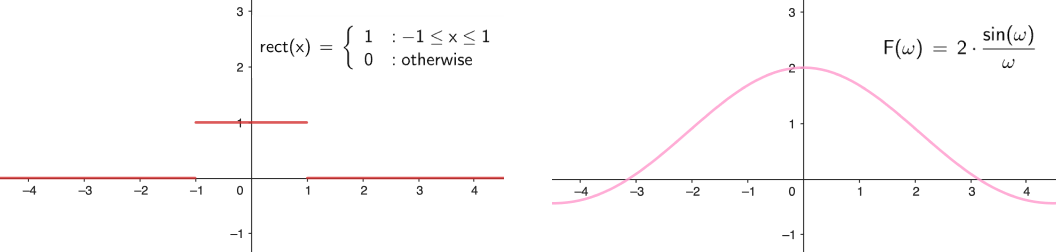
\includegraphics[width=0.8\linewidth]{img/example-fourier-trans.png}
	\caption{Rechteckfunktion und ihre Fourier-Transformation}
	\label{fig:fourier_transform}
\end{figure}

\noindent
Die Abbildung \ref{fig:fourier_transform} stellt die \( \text{rect}(x) \) Funktion und ihre
Fourier-Transformation, die als \( \text{sinc}(\omega) \) bezeichnet wird, dar. Die Nullstellen
\( \pm \pi, \pm 2 \pi, \pm 3 \pi, \dots \) der \( \text{sinc}(\omega) \) Funktion deuten darauf
hin, dass die \( \text{rect}(x) \) Funktion bei diesen Frequenzen keine Energie besitzt. Die
primäre Energie der Funktion liegt bei \( \omega=0 \). Beispiel adaptiert von
(\cite[Chapter~5 - Example~5.1]{hansen2014fourier}).



\subsubsection{Diskrete Fourier-Transformation}

Die diskrete Fourier-Transformation (DFT) stellt eine diskrete Variante der kontinuierlichen
Fourier-Transformation dar und wird speziell auf diskrete Signale angewendet. In digitalen
Systemen sind Signale typischerweise diskret und bestehen aus einzelnen Samples, weshalb die DFT
besonders relevant für solche Anwendungen ist. Die mathematische Definition der DFT ist
(\cite[Chapter~3]{hansen2014fourier}):

\[
	F(k) = \sum_{n=0}^{N-1} f(n) \cdot e^{-\frac{2\pi i}{N} kn}
\]

\noindent
\newline
Zur Veranschaulichung betrachten wir ein Code-Beispiel. Wir haben eine Funktion \(f(t)\) und unterteilen
diese in \(N\) Samples. Die DFT berechnet nun die Frequenzkomponenten des Signals. Die Abbildung
\ref{fig:dft_example} zeigt ein Beispiel für ein Signal \(f(t)\) mit \(N=5\) Samples.

\[ f(t) = 1.5 \cos(t) + 0.25 \sin(t) + 2 \sin(2t) + \sin(3t) \].


\begin{lstlisting}
import numpy as np
import matplotlib.pyplot as plt

def f(x):
    return 1.5 * np.cos(x) + 0.25 * np.sin(x) + 2 * np.sin(2*x) + np.sin(3*x)

N_SAMPLES = 5

x_curve = np.linspace(0, 2*np.pi, 100) # 100 Punkte zwischen 0 und 2pi
x_points = np.linspace(0, 2*np.pi, N_SAMPLES) # 5 Punkte zwischen 0 und 2pi

plt.plot(x_curve, f(x_curve))
plt.plot(x_points, f(x_points), 'o') # Plotte die 5 Punkte
\end{lstlisting}

\begin{figure}[h]
	\centering
	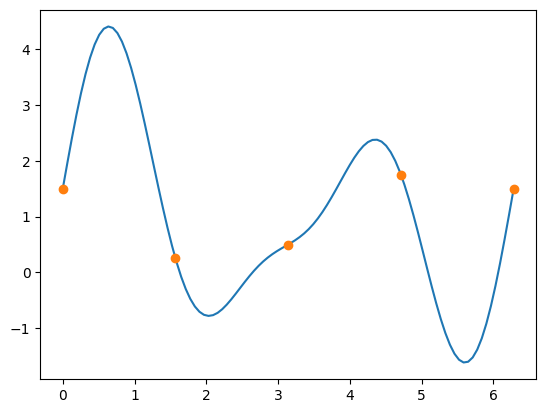
\includegraphics[width=0.60\linewidth]{img/dft.png}
	\caption{Funktion \( f(x) \) mit 5 Samples}
	\label{fig:dft_example}
\end{figure}

\noindent
Nun berechnen wir die DFT der 5 Samples. Dazu verwenden wir die \texttt{fft} Funktion aus der
\texttt{numpy} Bibliothek. Das Resultat ist ein Array mit \(N\) komplexen Zahlen. Die Tabelle
\ref{tab:dft_example_table} zeigt die Funktion \(f(x)\) und die DFT der 5 Samples.

\begin{lstlisting}
fhat = np.fft.fft(f(x_points), N_SAMPLES)
\end{lstlisting}

\begin{table}[h]
	\centering
	\begin{tabular}{|c|c|c|c|c|c|}
		\hline
		         & 0                & 1                & 2                & 3                & 4                \\
		\hline
		\(f(x)\) & 1.5              & 0.25             & 0.5              & 1.75             & 1.5              \\
		\hline
		dft      & \(5.50 + 0.00i\) & \(0.22 + 1.92i\) & \(0.78 - 0.45i\) & \(0.78 + 0.45i\) & \(0.22 - 1.92i\) \\
		\hline
	\end{tabular}
	\caption{\(f(x)\) und die DFT der 5 Samples}
	\label{tab:dft_example_table}
\end{table}

\noindent
Mit den Frequenzkomponenten der DFT können Signale manipuliert werden, etwa durch Filtern
bestimmter Frequenzbereiche. Um das ursprüngliche Signal wiederzuerlangen, wenden wir die inverse
DFT an. Die Formel der inversen DFT, welche das Signal rekonstruiert, lautet
(\cite[Chapter~3]{hansen2014fourier}):


\[
	f(n) = \frac{1}{N} \sum_{k=0}^{N-1} F(k) \cdot e^{\frac{2\pi i}{N} kn}
\]

\begin{lstlisting}
reconstructed_manual = np.zeros_like(x_points, dtype=np.complex128)

dt = x_points[1] - x_points[0] # Abstand zwischen zwei Punkten
T = N_SAMPLES * dt # Periode des Signals

for n in range(N_SAMPLES):
    # Rekonstruiert Signal mit Fourier-Koeffizienten, neg. Freq. bei n > N_SAMPLES/2.
    freq = n / (2*np.pi) if n <= N_SAMPLES//2 else (n - N_SAMPLES) / (2*np.pi)
    reconstructed_manual += fhat[n] * np.exp(1j * 2 * np.pi * freq * x)

reconstructed_manual = (reconstructed_manual / N_SAMPLES).real
reconstructed = np.fft.ifft(fhat).real # Rekonstruiertes Signal mit ifft
\end{lstlisting}

\begin{figure}[h]
	\centering
	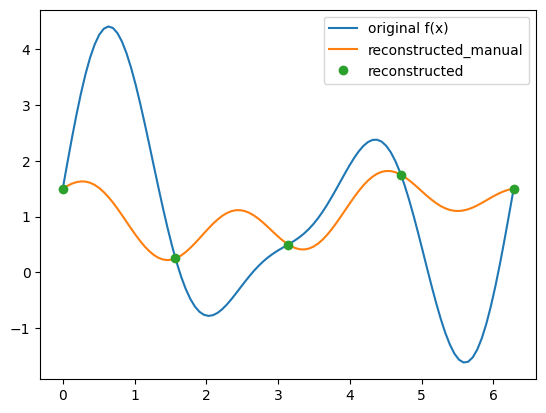
\includegraphics[width=0.60\linewidth]{img/dft_reconstructed.png}
	\caption{Rekonstruktion des Signals \(f(x)\)}
	\label{fig:dft_example_reconstructed}
\end{figure}

\noindent
\newline
Die Abbildung \ref{fig:dft_example_reconstructed} zeigt die ursprüngliche Funktion \(f(x)\) und die
rekonstruierte Funktionen \texttt{reconstructed (n=5)} und \texttt{reconstructed (n=nyquist)}.
Die Annäherung der mit der inversen DFT rekonstruierten Funktion an die ursprüngliche Funktion ist
bei \(n=5\) deutlich sichtbar. Bei \(n=nyquist\) ist die Annäherung nahezu perfekt, wenn nicht sogar
perfekt. Die Sampling-Rate bei der Nyquist angenäherten Funktion ist das Doppelte der höchsten
Frequenz des Signals. Das ist in diesem Fall \(2 \cdot 3 + 1 = 7\).

\subsubsection{Aliasing}
Aliasing tritt auf, wenn ein Signal bei einer nicht ausreichend hohen Samplingrate digital erfasst
wird, wodurch Frequenzen des Signals fehlinterpretiert werden können. Als allgemeines Beispiel wenn
ein Sinussignal mit einer Frequenz von 1200 Hz betrachtet wird und dieses mit einer Samplingrate
von nur 1000 Hz aufgenommen wurde, könnte das digitalisierte Signal so aussehen, als ob das
ursprüngliche Signal eine Frequenz von 200 Hz hätte. Das ist, als ob man ein sich schnell
drehendes Rad filmt und auf dem Video wirkt es, als würde es sich langsamer oder sogar rückwärts
drehen. Um solche Fehler zu verhindern, sollte die Samplingrate stets mindestens das
Doppelte der höchsten Frequenz des Signals betragen, ein Grundsatz, der als Nyquist-Kriterium
bekannt ist. (\cite[]{weitz2023fourier}).

\subsection{Spektrogramm}
Mit einem Verständnis der Grundlagen der Fourier-Analyse können wir die Bedeutung des Spektrogramms
erfassen. Ein Spektrogramm bietet eine visuelle Darstellung der verschiedenen Frequenzen, die in
einem Signal über die Zeit hinweg vorhanden sind. Ein Spektrogramm wird wie folgt definiert:

\begin{displayquote}
	''A spectrogram is a three-dimensional visualization of a signal’s amplitude over frequency and
	time. Many audio signals are comprised of multiple frequencies occurring simultaneously, with
	these frequencies often changing over time.'' (\cite[Chapter~15.2.1]{tarr2018hackaudio})
\end{displayquote}

\noindent
Im Bereich des Machine Learning, insbesondere bei der Spracherkennung, nimmt das Spektrogramm eine
zentrale Position ein. Die Fourier-Transformation eines Audiosignals in seine Frequenzkomponenten
resultiert in einem Verlust der zeitlichen Informationen durch die Anwendung der FFT. Für Aufgaben
wie die Spracherkennung ist es jedoch von grundlegender Bedeutung, nicht nur die im Signal
vorhandenen Frequenzen zu identifizieren, sondern auch den Zeitpunkt ihres Auftretens zu bestimmen.
Hier schafft das Spektrogramm Abhilfe, da es die zeitliche Abfolge der Frequenzen sichtbar macht.
Diese Fähigkeit ist insbesondere für das Erkennen der Sequenz gesprochener Wörter in einem Satz von
Bedeutung (\cite{chaudhary2020}). Somit verknüpft das Spektrogramm zeitliche und frequenzbezogene
Informationen, was es zu einem wichtigen Instrument für die Spracherkennung und andere Machine
Learning-Anwendungen macht. Abbildung \ref{fig:spectrogram} zeigt ein Beispiel eines Spektrogramms,
das im Rahmen dieser Arbeit entwickelt wurde. Das Spektrogramm wurde unter Verwendung der
Python-Bibliotheken \texttt{PyQt6} für die Echtzeit-Visualisierung und \texttt{soundevice} für den
Zugriff auf die Audio-Hardware generiert.

\begin{figure}[h]
	\centering
	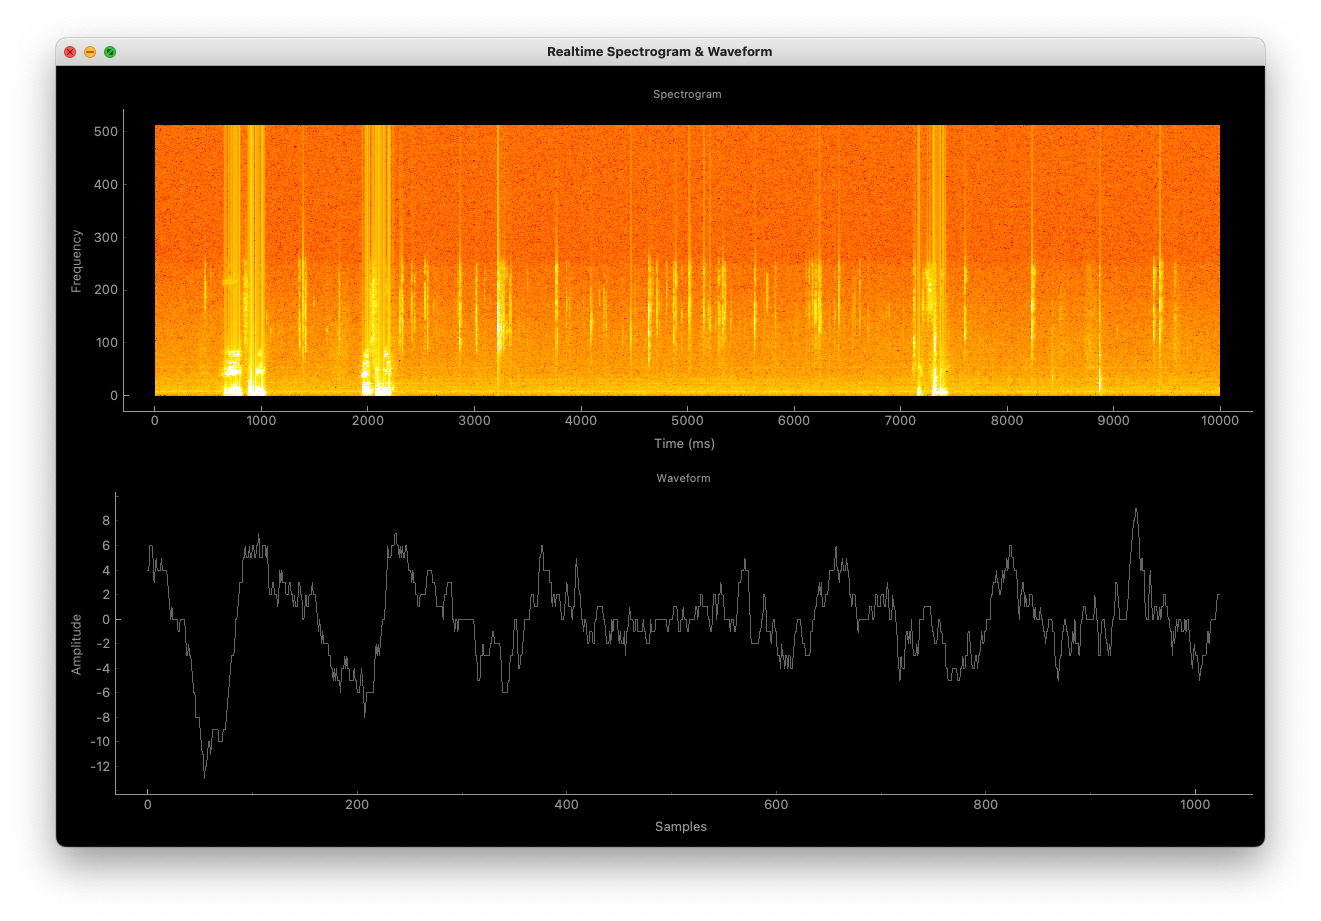
\includegraphics[width=0.73\linewidth]{img/spectrogram.png}
	\caption{Spektrogramm}
	\label{fig:spectrogram}
\end{figure}

\subsection{Machine Learning}
Dieses Kapitel erläutert die grundlegenden Konzepte von Machine Learning, die für die 
Spracherkennung relevant sind. Es fokussiert sich auf Deep Neural Networks (DNN), Convolutional 
Neural Networks (CNN) und Recurrent Neural Networks (RNN). (\cite{weidman2019deep})

\subsubsection{Neuronale Netze}
Unter Neuronalen Netzen versteht man im Allgemeinen eine Reihe von Berechnungen, die von der
Funktionsweise des menschlichen Gehirns inspiriert sind. Im Grunde sind es mathematische Modelle,
die aus einer Reihe von miteinander verbundenen Knoten bestehen, die als Neuronen bezeichnet werden.
Im einfachsten Fall bestehen Neuronen aus Inputs \(x_{1}, x_{2}, \dots, x_{n}\), Gewichten 
\(w_{1}, w_{2}, \dots, w_{n}\), einem Bias \(b\) einer Aktivierungsfunktion \(f\) und einem Output 
\(y\). Die Abbildung \ref{fig:neuron} zeigt ein einfaches Beispiel davon:

\begin{figure}[h]
	\centering
	\begin{tikzpicture}
		% Nodes for x1, x2
		\foreach \i/\y in {1/-1,2/-2} {
			\node[circle,fill=gray!30,minimum size=1cm] (x\i) at (0,\y) {$x_{\i}$};
			\node (w\i) at (2,\y) {$w_{\i}$};
			\draw[->] (x\i) -- (w\i) -- (4,-2.5);
		}
		
		% Nodes for xn
		\node[circle,fill=gray!30,minimum size=1cm] (xn) at (0,-4) {$x_{n}$};
		\node (wn) at (2,-4) {$w_{n}$};
		\draw[->] (xn) -- (wn) -- (4,-2.5);
	
		% Dots
		\node at (0,-3) {$\vdots$};
		\node at (2,-3) {$\vdots$};
	
		% Summation and Activation
		\node[circle,draw,minimum size=2cm] (sum) at (5,-2.5) {$\Sigma | f$};
		\node (activation) at (9,-2.5) {$f\left(b+\sum_{i=1}^{n}x_{i}\cdot w_{i}\right) = y$};
		\draw[->] (sum) -- (activation);
	
		% Bias
		\node (b) at (3,0) {$b$};
		\draw[->] (b) -- (sum);
	\end{tikzpicture}
	
	\caption{Neuronale Netze}
	\label{fig:neuron}

\end{figure}

\noindent
Neuronale Netze sind gut geeignet, um komplexe Probleme zu lösen, die nicht mit traditionellen
Algorithmen gelöst werden können. Ein Beispiel dafür ist die Spracherkennung oder auch die
Bilderkennung. Netzwerke werden trainiert, um die richtigen Gewichte \(w_{1}, w_{2}, \dots, w_{n}\)
und den Bias \(b\) zu finden, um die gewünschte Ausgabe zu erhalten. Um ein detailiertes Verständnis
von neuronalen Netzen zu erhalten, empfiehlt sich die Lektüre von (\cite{weidman2019deep}).

\subsubsection{Convolutional Neural Networks}
Convolutional Neural Networks (CNN) sind eine spezielle Art von neuronalen Netzen, die vor allem
in der Bilderkennung eingesetzt werden. Sie sind in der Lage, komplexe Muster in Bildern zu 
erkennen. In CNNs sind \textit{Convolutional Layers} zentral. Sie nutzen einen Filter, der über den 
Input gleitet und mit diesem verrechnet wird, wie Abbildung \ref{fig:convolution} zeigt.

\begin{figure}[h]
	\centering
	\begin{tikzpicture}[scale=0.6, every node/.style={scale=0.6}]
		% Input Image
		\matrix (input) [matrix of nodes, nodes in empty cells, nodes={draw, minimum size=1cm, anchor=center}]{
		5 & 3 & 1 & 0 & 9 \\
		12 & 4 & 1 & 0 & 2 \\
		5 & 3 & 1 & 0 & 2 \\
		5 & 21 & 1 & 0 & 1 \\
		0 & 0 & 1 & 0 & 9 \\
		};
		\node[below=0.5cm of input] {Input Image};
	
		% Filter
		\matrix (detector) [matrix of nodes, nodes in empty cells, nodes={draw, minimum size=1cm, anchor=center}, right=2cm of input]{
		1 & 0 & 1 \\
		29 & 1 & 0.5 \\
		0 & 1 & 1 \\
		};
		\node[below=0.5cm of detector] {Filter};
	
		% Output
		\matrix (map) [matrix of nodes, nodes in empty cells, nodes={draw, minimum size=1cm, anchor=center}, right=2cm of detector]{
		53. & 10. & 62.5 \\
		56.5 & 28.5 & 61.5 \\
		61.5 & 15.5 & 40.5 \\
		};
		\node[below=0.5cm of map] {Output};
	
		% Operators
		\node (conv) [circle, draw, gray, minimum size=1cm, right=0.5cm of input] {conv};
		\node (eq) [circle, draw, gray, minimum size=1cm, right=0.5cm of detector] {=};
	
		% Thicker border around the first 3x3 on the input
		\node[draw, thick, rectangle, fit={(input-1-1.north west) (input-3-3.south east)}, line width=1.5pt, inner sep=17pt] {};
	
	\end{tikzpicture}

	\caption{Convolution}
	\label{fig:convolution}

\end{figure}

\noindent
Bei CNNs sind die Gewichte \(w_{1}, w_{2}, \dots, w_{n}\) und der Bias \(b\) die Filter. 
Filter werden während des Trainings optimiert, um die gewünschte Ausgabe zu erhalten. Der grosse 
Vorteil gegenüber herkömmlichen neuronalen Netzen ist, dass die Gewichte geteilt werden können.
(\cite{weidman2019deep}) beschreibt CNNs wie folgt:

\begin{displayquote}
	''CNNs are the standard neural network architecture used for prediction when the input 
	observations are images, which is the case in a wide range of neural network applications.''
\end{displayquote}

\noindent
Speziell für CNNs sind die sogenannten \textit{Convolutional Layers}. Diese Layer bestehen aus
einem Filter, der über den Input von Links nach Rechts und von Oben nach Unten geschoben wird. 
Der Filter ist eine Matrix, die mit dem Input verrechnet wird. Die Abbildung \ref{fig:convolution} 
zeigt ein Beispiel einer Convolution.




\subsubsection{Recurrent Neural Networks}


\newpage \section{Stand der Forschung}
Der Stand der Forschung ist ein wichtiger Teil dieser Arbeit. Darin werden die wichtigsten 
zeitlichen Entwicklungen im Bereich der Spracherkennung dargestellt. Weiter werden die 
Sprachassistenten verglichen und die verwendeten Technologien aufgezeigt. Ein wichtiger Teil ist
die Funktionsweise vom Sprachassistent Siri. Apple veröffentlichte seinen Sprachassistenten 
im Jahr 2011 mit dem Release von iOS 5. Ebenfalls werden InApp Sprachassistenten im
Markt verglichen. Die Forschung im Bereich der Spracherkennung ist ein aktives Forschungsgebiet. 
Die Jahre 2010 bis 2020 haben laut (\cite{hannun2021history}) einen grossen Fortschritt in der 
Spracherkennung erlebt. Dieser Fortschritt ist vor allem auf die Verwendung von Deep Learning 
zurückzuführen. In der Allgemeinheit ist Spracherkennung vor allem durch die Sprachassistenten von 
Apple, Google und Amazon bekannt. 


\subsection{Zeitliche Entwicklung der Spracherkennung} 
Die Spracherkennung entwickelte sich von 2010 bis 2020 mit enormen Fortschritten. In der heutigen
Zeit wird die Spracherkennung in Form von Sprachassistenten wie Siri, Alexa und Google Assistant von
vielen Menschen genutzt. Die Nutzung der Sprachassistenten wird vor allem für Suchanfragen 
verwendet. Angesichts des Fortschritts der letzten Jahre stellt sich die Frage, was die Zukunft
bringen wird (\cite{hannun2021history}).

\noindent \newline
Die Abbildung \ref{fig:updated_timeline} zeigt eine Timeline der wichtigsten Entwicklungen im 
Zeitraum von 2010 bis 2020. Die Timeline wurde basierend auf der Timeline von 
(\cite{hannun2021history}) erstellt aber mit einem Zusatz für das Jahr 2020, welches die neuste 
Entwicklung von Facebook AI's wav2vec2 aufzeigt (\cite{baevski2020wav2vec}).

\begin{figure}[htb]
    \centering
    \begin{tikzpicture}[scale=1.5, every node/.style={scale=0.8}] 
        % Drawing the horizontal line
        \draw[->, thick] (0,0) -- (10,0);
        \foreach \x in {0,10} {
            \draw (\x,-0.1) -- (\x,0.1);
        }

		\foreach \x [count=\xi] in {2010,...,2020} {
			\draw (\xi-1,-0.1) -- (\xi-1,0.1); % draws the tick mark
			% \node[below] at (\xi-1,-0.2) {\x}; % labels the tick mark
		}

        % Labeling
        \node[align=center, below] at (0,-0.8) {2010};
        \node[align=center, below] at (10,-0.8) {2020};

        % Events
		\node[align=center, above] (kaldi) at (1.25,0.5) {Kaldi};
		\node[align=center, above] (hybrid) at (2.4,1) {Hybrid\\HMM/DNN};
		\node[align=center, above] (deepspeech) at (4.75,0.5) {Deep\\Speech};
		\node[align=center, above] (librispeech) at (5.5,1) {LibriSpeech};
		\node[align=center, above] (googlehome) at (6.7,1) {Google\\Home};
		\node[align=center, above] (humanlevel) at (7.75,0.75) {Human-level\\Switchboard};
		\node[align=center, above] (wav2vec2) at (10.0,0.75) {Facebook AI\\wav2vec2};
		\node[align=center, below] (applesiri) at (1.6,-0.8) {Apple Siri};
		\node[align=center, below] (amazonecho) at (4.55,-0.5) {Amazon Echo};
		\node[align=center, below] (encoder) at (5.8,-1.175) {Encoder-decoder\\models for ASR};
		\node[align=center, below] (deepspeech2) at (6.75,-0.5) {Deep Speech 2};
		\node[align=center, below] (googletransducer) at (9,-1) {Google streaming\\on-device transducer};

		% Lines to the events
		\draw (kaldi) -- (1.25,0.1);
		\draw (hybrid) -- (2.4,0.1);
		\draw (deepspeech) -- (4.75,0.1);
		\draw (librispeech) -- (5.5,0.1);
		\draw (googlehome) -- (6.7,0.1);
		\draw (humanlevel) -- (7.75,0.1);
		\draw (wav2vec2) -- (10.0,0.1);
		\draw (applesiri) -- (1.6,-0.1);
		\draw (amazonecho) -- (4.55,-0.1);
		\draw (encoder) -- (5.8,-0.1);
		\draw (deepspeech2) -- (6.75,-0.1);
		\draw (googletransducer) -- (9,-0.1);
    \end{tikzpicture}
    \caption{Timeline of Speech Recognition Developments (2010-2020)}
	\label{fig:updated_timeline} % for later references
\end{figure}

\noindent \newline

\noindent \newline
Deep Learning hat zum grossen Teilen die Spracherkennung revolutioniert, insbesondere durch die 
Sammlung grosser transkribierter Datensätze und Fortschritte in der Hardware. Spätestens seit 
(\textit{Deep Speech}) sind Fähigkeiten der akustischen Sprachmodelle mit denen von Menschen
vergleichbar (\cite{hannun2021history}). 

\noindent \newline
Als offene Vorhersage für die Zukunft der Spracherkennung bezieht sich (\cite{hannun2021history}) 
auf die Entwicklung bis 2030. Bis 2030 wird die Spracherkennungs-Forschung eine Verlagerung zu 
self-supervised Modellen und On-Device-Training erleben, wobei der Fokus auf kleine sparsame Modelle
und personalisierten Modellen liegt. Die Wortfehlerrate wird weiter sinken, während die 
Sprachqualität steigt (\cite{hannun2021history}).

\subsection{Komparative Analyse von Sprachassistenten}
TODO: - (\cite{matarneh2017speechrecognition}) bietet eine komparative Analyse von 
Sprachassistenten. Die Analyse "Voice control implementation may be conditionally divided into 
parts: speech, recognition, translation, and execution of commands (Fig. 1)."

\subsection{Funktionsweise von Siri}
Die Implementation von Siri ist nicht öffentlich zugänglich, aber Apple selbst dokumentiert 
das Grundlegende Konzept von Siri sehr detailliert. Der Beitrag ``Hey Siri: An On-device DNN-powered 
Voice Trigger for Apple’s Personal Assistant'' \cite{siri2017hey} von der ML Research Group von 
Apple gibt einen sehr detaillierten Einblick in die Funktionsweise von Siri. Siri besteht aus
diversen Komponenten, welche mehrheitlich in der Cloud laufen. ``Most of the implementation of Siri 
is in the Cloud, including the main automatic speech recognition, the natural language 
interpretation and the various information services.'' (\cite{siri2017hey}). Der Trigger von Siri
läuft jedoch auf dem Gerät selbst. Um diesen geht es im wesentlichen in diesem Kapitel.

\noindent \newline
Siri verwendet für den Voice Trigger ein Deep Neural Network (DNN) um das akustische Muster jedes 
Frames in eine Verteilung von Wahrscheinlichkeiten für jeden Phonem zu übersetzen. Die Phoneme sind 
die Bausteine der akustischen Sprache. Aus den Wahrscheinlichkeiten wird in einen zeitlichen 
Integrationsprozess bestimmt, wie sicher es ist, dass das Gesagte 'Hey Siri' war.

\noindent \newline
Das Mikrofon des Geräts wandelt das Audiosignal in einen kontinuierlichen Stream von 16000 Samples 
pro Sekunde um. Diese Samples werden anschliessend durch eine Spektralanalyse in eine Abfolge von 
Frames transformiert, wobei jeder dieser Frames das Spektrum von ungefähr 0,01 Sekunden beschreibt.
Zwanzig Frames, die sich über 0,2 Sekunden erstrecken, werden dann als Eingabe für das DNN 
verwendet.
 
e ....


\noindent \newline
TODO: Offenlegung der Funktionsweise von Siri. Wie funktioniert Siri? Als Beispiel eines OS 
übergreifenden Sprachassistenten.
(\cite{siri2017hey}) und (\cite{apple2023voice}) 

\begin{itemize}
    \item Untersuchung und Darstellung der Funktionsweise von Siri.
    \item Nutzung der Quellen \cite{siri2017hey} und \cite{apple2023voice} zur detaillierten 
    Erklärung von Siris Arbeitsweise.
    \item Überprüfen der Links für zusätzliche Informationen:
    \begin{itemize}
        \item \url{https://machinelearning.apple.com/research/hey-siri}
        \item \url{https://machinelearning.apple.com/research/voice-trigger}
    \end{itemize}
\end{itemize}

\subsection{In App Sprachsteuerung}
TODO: Siri bietet API für In App Sprachsteuerung. Wie funktioniert das? Wie kann das verwendet.
Keine eigenen Triggerwörter möglich. Gibt es alternativen?

\subsection{Marktanalyse - Benchmarking}

die machen es komerziell, ich mache es open source
https://picovoice.ai/platform/porcupine/ 

\subsection{Diskussion}



\newpage \section{Ideen und Konzepte}
Dieses Kapitel beschreibt die Ideen und Konzepte, die für die Umsetzung der Arbeit verwendet
werden. Es wird auch auf die verwendeten Technologien eingegangen.

Die Grob Idee ist es im wesentlichen, ein eigenes Modell zu trainieren, welches Triggerwörter
erkennt. Dazu wird ein Datensatz erstellt, welcher die Triggerwörter, sowie andere Wörter
enthält.

In einem ersten Schritt wird ein eigenes Modell trainiert, welches Triggerwörter erkennt.
Es gibt aber auch die Möglichkeit, ein bereits vortrainiertes Modell zu verwenden. Dieses Kapitel
\subsection{Einleitung}
\begin{itemize}
    \item Kurze Wiederholung des Problems und der Vision für Ihr Projekt.
    \item Einführung in die Ideen und Konzepte, die Sie in Betracht ziehen, um dieses Ziel zu erreichen.
\end{itemize}

\subsection{Grundlegende Idee}
\begin{itemize}
    \item Erklärung, wie eine integrierte Spracherkennung den Benutzererfahrungen in mobilen Apps verbessern könnte.
    \item Beispiel: Automatisierte To-Do-Liste-Einträge durch Sprachbefehle.
\end{itemize}

\subsection{Skizzenhafte Lösungsansätze}
\begin{itemize}
    \item Machine Learning: Verwendung von bereits trainierten Modellen oder Aufbau eigener Modelle zur Triggerwort-Erkennung.
    \item Cloud vs. Edge Computing: Ob die Spracherkennung in der Cloud oder direkt auf dem Gerät erfolgen sollte.
    \item Integration: SDKs oder APIs, die Entwicklern helfen, die Spracherkennungsfunktionalität in ihre Apps zu integrieren.
\end{itemize}

\subsection{Systemarchitektur}
\begin{itemize}
    \item Überlegungen zur Systemarchitektur: Ist ein monolithisches System oder eine Microservice-Architektur sinnvoller?
    \item Vorteile und Herausforderungen beider Ansätze im Kontext der Spracherkennung.
\end{itemize}

\subsection{Alternative Ansätze}
\begin{itemize}
    \item Untersuchung anderer Technologien oder Ansätze zur Spracherkennung, z.B. regelbasierte Systeme im Vergleich zu Machine Learning.
    \item Warum Sie sich für einen bestimmten Ansatz entschieden haben oder warum Sie einen anderen verworfen haben.
\end{itemize}

\subsection{Mögliche Problempunkte}
\begin{itemize}
    \item Datenschutz: Wie wird die Privatsphäre der Benutzer gewahrt?
    \item Effizienz: Wie kann sichergestellt werden, dass die Spracherkennung schnell und akkurat ist?
    \item Integration: Wie kann die Kompatibilität mit einer Vielzahl von Apps und Plattformen gewährleistet werden?
\end{itemize}

\subsection{Erste Überlegungen zu Tools und Technologien}
\begin{itemize}
    \item Welche Programmiersprachen oder Frameworks könnten verwendet werden?
    \item Eventuelle Betrachtung von Open-Source-Optionen für Spracherkennung.
\end{itemize}

\subsection{Zusammenfassung und Ausblick}
\begin{itemize}
    \item Ein kurzer Überblick über die in diesem Kapitel vorgestellten Ideen und Konzepte.
    \item Ein Vorgeschmack darauf, wie diese Konzepte in den kommenden Kapiteln weiter verfolgt werden.
\end{itemize}


....

\newpage \section{Methoden}
Am besten dieses Paper verwenden (\cite{choi2018tutorial}).

\subsection{Vorgehensmodell}
\begin{itemize}
    \item Auswahl des passenden Vorgehensmodells zur Integration einer Spracherkennungsfunktion, z.B. iteratives Modell.
    \item Verweis auf den konkreten Terminplan mit Meilensteinen spezifisch für die Spracherkennungs-Integration (im Kapitel 5 oder im Anhang).
\end{itemize}

\subsection{Forschungsmethoden (falls anwendbar)}
\begin{itemize}
    \item Erwägung von Benutzertests, um zu prüfen, wie intuitiv und effizient die Spracherkennungsfunktion ist.
    \item Interviews mit potenziellen Nutzern der App, um ihre Anforderungen und Erwartungen in Bezug auf Spracherkennung zu verstehen.
\end{itemize}

\subsection{Technische Evaluierung}
\begin{itemize}
    \item Vergleich verschiedener Spracherkennungs-APIs oder Frameworks hinsichtlich Genauigkeit, Latenz, Sprachunterstützung und Kosten.
    \item Technische Tests zur Prüfung der Performance und Genauigkeit der gewählten Spracherkennungslösung.
\end{itemize}

\subsection{Integrationsmethode}
\begin{itemize}
    \item Beschreibung der geplanten Techniken zur Integration, z.B. Einbindung über API, Implementierung bestimmter Bibliotheken oder Nutzung nativer App-Funktionen.
    \item Diskussion über potenzielle Herausforderungen bei der Integration und wie sie angegangen werden sollen.
\end{itemize}

\subsection{Teststrategie}
\begin{itemize}
    \item Entwurf einer Teststrategie speziell für die Spracherkennungsfunktion: Testen unter verschiedenen Bedingungen (z.B. Hintergrundgeräusche, verschiedene Sprachen und Akzente).
    \item Verweis darauf, dass die eigentliche Testdurchführung in einem anderen Kapitel oder Dokument beschrieben ist.
\end{itemize}

\newpage \section{Realisierung}
Das Problem dieser Arbeit ist im wesentlichen die Erkennung von Triggerwörtern innerhalb
des Kontext einer App. Grundsätzlich ist es unüblich, dass mobile Apps eine
integrierte Sprachsteuerungsfunktion anbieten.


\subsection{Google Cloud Platform}
TODO: Google Cloud Platform um Datensätze zu hosten auf Sorage Bucket. 
TODO: Recorder Webseite für Aufnahme von Sprachsamples
(\cite{warden2018speech}

In den Sample zu VoiceCommands wird eine Recorder Webseite angeboten, mit welcher Sprachsamples
aufgenommen werden können. Selbsterstellen einer kleinen Seite Hosting dieser Webseite auf GCP
https://github.com/petewarden/open-speech-recording/tree/master

Fork 
(\cite{warden2018speech})


\subsubsection{Recorder Webseite}

\subsection{Datensatz}
Um ein Modell zu trainieren, welches Triggerwörter erkennt, wird ein Datensatz benötigt.

\subsubsection{Datensatz 'other}
Am besten von Datenset (\cite{warden2018speech})
\begin{itemize}
    \item Datenset von Mozilla Common Voice
    \item Datenset von Google Speech Commands
\end{itemize}

\subsubsection{Datensatz 'hey-fooby'}
\begin{itemize}
    \item TODO: Recorder Webseite für Aufnahme von Sprachsamples
    \item Synthetische Sprachsamples mit verschiedenen Stimmen Geräuschen und Hintergrundgeräuschen
\end{itemize}

\subsection{Modell}
\begin{itemize}
    \item Auswahl des Modells
    \item Auswahl der Hyperparameter
    \item Training des Modells
    \item Evaluation des Modells
\end{itemize}

\subsubsection{Modell 'CNN'}
\begin{itemize}
    \item Aufbau des Modells 
    \item TODO: Beschreibung des Modells
\end{itemize}

\subsubsection{Modell 'RNN'}
\begin{itemize}
    \item Aufbau des Modells 
    \item TODO: Beschreibung des Modells

\end{itemize}



\newpage \section{Evaluation und Validation}
Das Problem dieser Arbeit ist im wesentlichen die Erkennung von Triggerwörtern innerhalb
des Kontext einer App. Grundsätzlich ist es unüblich, dass mobile Apps eine
integrierte Sprachsteuerungsfunktion anbieten.

\newpage \section{Ausblick}
Das Problem dieser Arbeit ist im wesentlichen die Erkennung von Triggerwörtern innerhalb
des Kontext einer App. Grundsätzlich ist es unüblich, dass mobile Apps eine
integrierte Sprachsteuerungsfunktion anbieten.

\newpage \section{Anhang}
\subfile{projectmanagement.tex}

\clearpage
% Glossar
\addcontentsline{toc}{section}{Glossar}
\printglossary[type=\acronymtype,title=Akronyme]
\printglossary[title=Glossar]
% Verzeichnisse
\addcontentsline{toc}{section}{Abbildungsverzeichnis}
\listoffigures
\addcontentsline{toc}{section}{Tabellenverzeichnis}
\listoftables
\printbibliography[title=Literaturverzeichnis, heading=bibintoc]



%       %%%%%   %    %   %%%
%       %       % %  %   %   %
%       %%%%    %  % %   %    %
%       %       %   %%   %   %
%       %%%%%   %    %   %%%


\newpage
\pagecolor{ba-gray}
\afterpage{\nopagecolor}
\blankpage

\newpage

\section*{Aufgabenstellung}
Integration von Sprachsteuerungstechnologien in Mobile Apps, insbesondere zur Erkennung
von Triggerwörtern.

\section*{Projektteam}
\begin{itemize}
	\item Student:in: Rubén Nuñez
	\item Betreuer:in: Herzog
	\item Firma: Bitforge AG
\end{itemize}

\section*{Auftraggeber}
\begin{itemize}
	\item Firma: Bitforge AG
	\item Ansprechperson: Stefan Reinhard
	\item Funktion: Head of Mobile
	\item Adresse: Zeughausstrasse 39, 8004 Zürich
	\item Telefon: +41 55 211 02 41
	\item E-Mail: stefan.reinhard@bitforge.ch
	\item Website: www.bitforge.ch
\end{itemize}

\section*{Sonstige Bemerkungen}
Grundkenntnisse in Machine Learning, speziell im Bereich der Spracherkennung, sowie
Erfahrung mit entsprechenden APIs sind erforderlich.

\end{document}
